\documentclass{beamer}
\usepackage[utf8]{inputenc}

\usetheme{Madrid}
\usecolortheme{default}
\usepackage{amsmath,amssymb,amsfonts,amsthm}
\usepackage{txfonts}
\usepackage{tkz-euclide}
\usepackage{listings}
\usepackage{adjustbox}
\usepackage{array}
\usepackage{tabularx}
\usepackage{gvv}
\usepackage{lmodern}
\usepackage{circuitikz}
\usepackage{tikz}
\usepackage{graphicx}

\setbeamertemplate{page number in head/foot}[totalframenumber]
\usepackage[T1]{fontenc}
\usepackage{tcolorbox}
\tcbuselibrary{minted,breakable,xparse,skins}

\definecolor{bg}{gray}{0.95}
\DeclareTCBListing{mintedbox}{O{}m!O{}}{%
  breakable=true,
  listing engine=minted,
  listing only,
  minted language=#2,
  minted style=default,
  minted options={%
    linenos,
    gobble=0,
    breaklines=true,
    breakafter=,,
    fontsize=\small,
    numbersep=8pt,
    #1},
  boxsep=0pt,
  left skip=0pt,
  right skip=0pt,
  left=25pt,
  right=0pt,
  top=3pt,
  bottom=3pt,
  arc=5pt,
  leftrule=0pt,
  rightrule=0pt,
  bottomrule=2pt,
  toprule=2pt,
  colback=bg,
  colframe=orange!70,
  enhanced,
  overlay={%
    \begin{tcbclipinterior}
    \fill[orange!20!white] (frame.south west) rectangle ([xshift=20pt]frame.north west);
    \end{tcbclipinterior}},
  #3,
}

% Code style
\lstset{
    language=C,
    basicstyle=\ttfamily\small,
    keywordstyle=\color{blue},
    stringstyle=\color{orange},
    commentstyle=\color{green!60!black},
    numbers=left,
    numberstyle=\tiny\color{gray},
    breaklines=true,
    showstringspaces=false,
}

%------------------------------------------------------------
% Title info
\title %optional
{4.2.16}
\date{October 1 , 2025}
\author % (optional)
{EE25BTECH11018 - Darisy Sreetej}

\begin{document}

\frame{\titlepage}

\begin{frame}{Question}
Find the equation of the plane passing through the points having position vectors $\hat{i}+\hat{j}-2\hat{k},2\hat{i}-\hat{j}+\hat{k},\hat{i}+2\hat{j}+\hat{k}$.Write the equation of the plane passing through a point $(2, 3, 7)$ and parallel to the plane obtained above. Hence, find the distance between the two parallel planes. 
\end{frame}
\begin{frame}{Formula}
The distance between the parallel planes is given by 
\begin{align}
\text{Distance} = \frac{\abs{d_1 - d_2}}{\norm{\vec{n}}}
\end{align}
where $\vec{n}^\top\vec{x}=d_1$ and $\vec{n}^\top\vec{x}=d_2$ are the parallel planes
\end{frame}
\begin{frame}
    \begin{table}[H]
	\centering
	\caption{}
	\begin{tabular}{|c|c|}
\hline
\textbf{Name} & \textbf{Value} \\ \hline
$\vec{A}$ & $\myvec{2 & 1 \\0 & 3}$ \\ \hline
\end{tabular}

	\label{}
\end{table}
\end{frame}
\begin{frame}{Obtaining the plane}
Let the equation of plane be
\begin{align}
	\vec{n}^\top\vec{x}=C_1
\end{align}
A,B,C satisfies this equation,
\begin{align}
	\vec{n}^\top\vec{A}=C_1,
	\vec{n}^\top\vec{B}=C_1,
	\vec{n}^\top\vec{C}=C_1
\end{align}
\begin{align}
	\myvec{\vec{A}\\\vec{B}\\\vec{C}}^\top\vec{n}=\myvec{C_1\\C_1\\C_1}
\end{align}
Using augmented matrix,
\begin{align}
	\augvec{3}{1}{1&1&-2&C_1\\2&-1&1&C_1\\1&2&1&C_1}
\end{align}
$R_2=R_2-2R_1$\\
$R_3=R_3-R_1$
\end{frame}
\begin{frame}
\begin{align}
	\augvec{3}{1}{1&1&-2&C_1\\0&-3&5&-C_1\\0&1&3&0}
\end{align}
$R_2 \Longleftrightarrow R_3$
\begin{align}
	\augvec{3}{1}{1&1&-2&C_1\\0&1&3&0\\0&-3&5&-C_1}
\end{align}
$R_3=R_3+3R_2$
\begin{align}
	\augvec{3}{1}{1&1&-2&C_1\\0&1&3&0\\0&0&14&-C_1}
\end{align}
\begin{align}
	14z+C_1=0\implies z=\frac{-C_1}{14} 
\end{align}
\begin{align}
	y+3z=0\implies y=\frac{3C_1}{14}
\end{align}
\end{frame}
\begin{frame}
\begin{align}
	x+y-2z=C_1\implies x=\frac{9C_1}{17}
\end{align}
Let $C_1=14$
\begin{align}
	\vec{n}=\myvec{9\\3\\-1},C_1=14
\end{align}
Equation of the plane 
\begin{align}
    \myvec{9\\3\\-1}^\top\vec{x}=14
\end{align}
\end{frame}
\begin{frame}{Obtaining the Parallel plane}
For finding parallel plane passing through P ,
\begin{align}
	\vec{n}^\top\vec{x}=C_2
\end{align}
\begin{align}
	\vec{n}^\top\vec{P}=C_2
\end{align}
\begin{align}
	C_2=\myvec{9&3&-1}\myvec{2\\3\\7}
\end{align}
\begin{align}
	C_2=20
\end{align}
Equation of plane parallel to given plane passing through point P is
\begin{align}
	\myvec{9\\3\\-1}^\top\vec{x}=20
\end{align}
\end{frame}
\begin{frame}{Distance between the planes}
    The $2$ planes obtained are parallel since their normal vectors are the same\\
The normal vector of the planes $\vec{n}$
\begin{align}
\vec{n} = \myvec{9 \\ 3 \\ -1}
\end{align}

The distance between the planes is given by this formula
\begin{align}
\text{Distance} = \frac{\abs{d_1 - d_2}}{\norm{\vec{n}}}
\end{align}

Where $d_1 = 14$ and $d_2 = 20$

\begin{align}
{\norm{\vec{n}}} = \brak{\sqrt{\brak{9}^2 + \brak{3}^2 + \brak{-1}^2}} = \sqrt{91}
\end{align}
Substituting these values in the distance formula, we get
\end{frame}
\begin{frame}
    \begin{align}
\therefore \text{Distance} = \frac{\abs{14-20}}{\sqrt{91}}
\end{align}
\begin{align}
\text{Distance} = \frac{6}{\sqrt{91}}
\end{align}
Therefore, the distance between the planes is $\frac{6}{\sqrt{91}}$
\end{frame}

\begin{frame}{Plot}
    \centering
    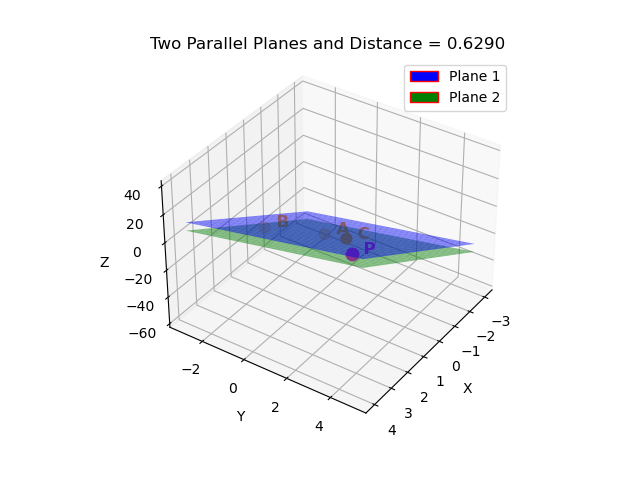
\includegraphics[width=3\columnwidth, height=0.8\textheight, keepaspectratio]{figs/fig.png}     
\end{frame}

\begin{frame}[fragile]
    \frametitle{C Code }
    \begin{lstlisting}[language=C]
#include <stdio.h>
#include <math.h>

void plane_from_points(double P1[3], double P2[3], double P3[3], double coeff[4]) {
    coeff[0] = (P2[1]-P1[1])*(P3[2]-P1[2]) - (P2[2]-P1[2])*(P3[1]-P1[1]);
    coeff[1] = (P2[2]-P1[2])*(P3[0]-P1[0]) - (P2[0]-P1[0])*(P3[2]-P1[2]);
    coeff[2] = (P2[0]-P1[0])*(P3[1]-P1[1]) - (P2[1]-P1[1])*(P3[0]-P1[0]);
    coeff[3] = -(coeff[0]*P1[0] + coeff[1]*P1[1] + coeff[2]*P1[2]);
}

void parallel_plane_through_point(double coeff[4], double Q[3], double coeff2[4]) {
    coeff2[0] = coeff[0];
    
    \end{lstlisting}
\end{frame}
\begin{frame}[fragile]
    \frametitle{C Code }
    \begin{lstlisting}[language=C]
coeff2[1] = coeff[1];
    coeff2[2] = coeff[2];
    coeff2[3] = -(coeff2[0]*Q[0] + coeff2[1]*Q[1] + coeff2[2]*Q[2]);
}

double norm(double *n) {
    return sqrt(n[0]*n[0] + n[1]*n[1] + n[2]*n[2]);
}

double plane_distance(double *n, double d1, double d2) {
    double num = fabs(d1 - d2);
    double denom = norm(n);
    return num / denom;
}
     \end{lstlisting}
\end{frame}
\begin{frame}[fragile]
    \frametitle{Python + C Code }
    \begin{lstlisting}[language=Python]
import ctypes
import numpy as np
import matplotlib.pyplot as plt

lib = ctypes.CDLL("./plane_distance.so")  

lib.plane_from_points.argtypes = [
    ctypes.POINTER(ctypes.c_double),
    ctypes.POINTER(ctypes.c_double),
    ctypes.POINTER(ctypes.c_double),
    ctypes.POINTER(ctypes.c_double)
]

lib.parallel_plane_through_point.argtypes = [
    ctypes.POINTER(ctypes.c_double),
    ctypes.POINTER(ctypes.c_double),
    ctypes.POINTER(ctypes.c_double)
]
    \end{lstlisting}
\end{frame}

\begin{frame}[fragile]
    \frametitle{Python + C code}

    \begin{lstlisting}[language=Python]
lib.plane_distance.argtypes = [
    ctypes.POINTER(ctypes.c_double),
    ctypes.c_double,
    ctypes.c_double
]
lib.plane_distance.restype = ctypes.c_double

A = [1, 1, -2]  # Given vector A
B = [2, -1, 1]  # Given vector B
C = [1, 2, 1]   # Given vector C
P = [2, 3, 7]   # Point P for the parallel plane

A_c = (ctypes.c_double * 3)(*A)
B_c = (ctypes.c_double * 3)(*B)
C_c = (ctypes.c_double * 3)(*C)
P_c = (ctypes.c_double * 3)(*P)

coeff1 = (ctypes.c_double * 4)()
    \end{lstlisting}
\end{frame}

\begin{frame}[fragile]
    \frametitle{Python + C code}

    \begin{lstlisting}[language=Python]
lib.plane_from_points(A_c, B_c, C_c, coeff1)
plane1 = np.array(coeff1[:])

coeff2 = (ctypes.c_double * 4)()
lib.parallel_plane_through_point(coeff1, P_c, coeff2)
plane2 = np.array(coeff2[:])

a, b, c, d1 = plane1
a2, b2, c2, d2 = plane2

n = np.array([a, b, c], dtype=np.double)
dist = lib.plane_distance(n.ctypes.data_as(ctypes.POINTER(ctypes.c_double)), d1, d2)
print(f"Distance between planes: {dist:.4f}")

xx, yy = np.meshgrid(np.linspace(-2, 3, 30), np.linspace(-2, 4, 30))
zz1 = (-d1 - a * xx - b * yy) / c
zz2 = (-d2 - a2 * xx - b2 * yy) / c2

    \end{lstlisting}
\end{frame}
\begin{frame}[fragile]
    \frametitle{Python + C code}

    \begin{lstlisting}[language=Python]
fig = plt.figure()
ax = fig.add_subplot(111, projection='3d')
ax.view_init(elev=25, azim=45)

ax.plot_surface(xx, yy, zz1, alpha=0.5, color='blue')
ax.plot_surface(xx, yy, zz2, alpha=0.5, color='green')
points = np.array([A, B, C, P])
labels = ["A", "B", "C", "P"]
for (x, y, z), label in zip(points, labels):
    ax.scatter(x, y, z, color='red', s=50)
    ax.text(x, y, z, label, color='black')

ax.set_xlabel("X")
ax.set_ylabel("Y")
ax.set_zlabel("Z")
ax.set_title(f"Two Planes and Distance = {dist:.4f}")
plt.show()
      \end{lstlisting}
\end{frame}
\begin{frame}[fragile]
    \frametitle{Python code}
    \begin{lstlisting}[language=Python]
import numpy as np
import matplotlib.pyplot as plt
from matplotlib.patches import Patch

def plane_from_points(A, B, C):
    AB = np.array(B) - np.array(A)
    AC = np.array(C) - np.array(A)
    n = np.cross(AB, AC)
    d = -np.dot(n, A)
    return n, d

def parallel_plane_through_point(n, d, P):
    d_new = -np.dot(n, P)
    return n, d_new

def plane_distance(n, d1, d2):
    return abs(d1 - d2) / np.linalg.norm(n)

    \end{lstlisting}
\end{frame}

\begin{frame}[fragile]
    \frametitle{Python code}

    \begin{lstlisting}[language=Python]
# Given points
A = [1, 1, -2]
B = [2, -1, 1]
C = [1, 2, 1]
P = [2, 3, 7]

# Calculate plane coefficients
n1, d1 = plane_from_points(A, B, C)
n2, d2 = parallel_plane_through_point(n1, d1, P)
dist = plane_distance(n1, d1, d2)
print(f"Distance between planes: {dist:.4f}")

# Create mesh grid for plotting planes
xx, yy = np.meshgrid(np.linspace(-3, 4, 30), np.linspace(-3, 5, 30))
zz1 = (-d1 - n1[0]*xx - n1[1]*yy) / n1[2]
zz2 = (-d2 - n2[0]*xx - n2[1]*yy) / n2[2]

           \end{lstlisting}
\end{frame}
\begin{frame}[fragile]
    \frametitle{Python code}

    \begin{lstlisting}[language=Python]
# Plot setup
fig = plt.figure()
ax = fig.add_subplot(111, projection='3d')
ax.view_init(elev=30, azim=60)

# Plot planes with legend
ax.plot_surface(xx, yy, zz1, alpha=0.5, color='blue', label='Plane 1')
ax.plot_surface(xx, yy, zz2, alpha=0.5, color='green', label='Plane 2')

# Plot points directly (no legend entry)
ax.scatter(*zip(*[A, B, C]), color='orange', s=60)
ax.scatter(*P, color='magenta', s=80)
# Mark points clearly with labels
for point, label, color in zip([A, B, C, P], ["A", "B", "C", "P"], ['orange', 'orange', 'orange', 'magenta']):
    ax.text(point[0], point[1], point[2], f'  {label}', color=color, fontsize=12, fontweight='bold')
    \end{lstlisting}
\end{frame}
\begin{frame}[fragile]
    \frametitle{Python code}

    \begin{lstlisting}[language=Python]
# Create legend only for planes using proxy artists
legend_elements = [
    Patch(facecolor='blue', edgecolor='r', label='Plane 1'),
    Patch(facecolor='green', edgecolor='r', label='Plane 2'),
]

ax.legend(handles=legend_elements, loc='best')

ax.set_xlabel("X")
ax.set_ylabel("Y")
ax.set_zlabel("Z")
ax.set_title(f"Two Parallel Planes and Distance = {dist:.4f}")

plt.show()
\end{lstlisting}
\end{frame}
\end{document}
